%%%%%%%%%%%%%%%%%%%%%%%%%%%%%%%%%%%%%%%%%
% Beamer Presentation
% LaTeX Template
% Version 1.0 (10/11/12)
%
% This template has been downloaded from:
% http://www.LaTeXTemplates.com
%
% License:
% CC BY-NC-SA 3.0 (http://creativecommons.org/licenses/by-nc-sa/3.0/)
%
%%%%%%%%%%%%%%%%%%%%%%%%%%%%%%%%%%%%%%%%%

%----------------------------------------------------------------------------------------
%	PACKAGES AND THEMES
%----------------------------------------------------------------------------------------

\documentclass[9pt]{beamer}
\usepackage{CJK}
\usepackage{ctex}
\usepackage{graphicx}
\usepackage{subfigure}
\usepackage{longtable}
\usepackage{rotating}
\usepackage{multirow}
\usepackage{algorithm}
\usepackage{algorithmic}
\usepackage{mathtools}
\usepackage{animate}
\usepackage{array}
%\usepackage{media9}
%% A LATEX package for embedding interactive Adobe Flash (SWF) and 3D files (Adobe U3D & PRC) as well as video and sound files or streams (FLV, MP4/H.246, MP3) into PDF documents with Adobe Reader-9/X
%compatibility.
\renewcommand{\algorithmicrequire}{\textbf{Input:}}   %Use Input in the format of Algorithm
\renewcommand{\algorithmicensure}{\textbf{Output:}}  %UseOutput in the format of Algorithm
\newcommand{\e}[1]{\ensuremath{\times 10^{#1}}}
%\mode<presentation>{\usetheme{Madrid}}

\mode<presentation> {

% The Beamer class comes with a number of default slide themes
% which change the colors and layouts of slides. Below this is a list
% of all the themes, uncomment each in turn to see what they look like.

%\usetheme{default}
%\usetheme{AnnArbor}
%\usetheme{Antibes}
%\usetheme{Bergen}
%\usetheme{Berkeley}
%\usetheme{Berlin}
%\usetheme{Boadilla}
%\usetheme{CambridgeUS}
%\usetheme{Copenhagen}
%\usetheme{Darmstadt}
%\usetheme{Dresden}
%\usetheme{Frankfurt}
%\usetheme{Goettingen}
%\usetheme{Hannover}
%\usetheme{Ilmenau}
%\usetheme{JuanLesPins}
%\usetheme{Luebeck}
\usetheme{Madrid}
%\usetheme{Malmoe}
%\usetheme{Marburg}
%\usetheme{Montpellier}
%\usetheme{PaloAlto}
%\usetheme{Pittsburgh}
%\usetheme{Rochester}
%\usetheme{Singapore}
%\usetheme{Szeged}
%\usetheme{Warsaw}

% As well as themes, the Beamer class has a number of color themes
% for any slide theme. Uncomment each of these in turn to see how it
% changes the colors of your current slide theme.

%\usecolortheme{albatross}
\usecolortheme{beaver}
%\usecolortheme{beetle}
%\usecolortheme{crane}
%\usecolortheme{dolphin}
%\usecolortheme{dove}
%\usecolortheme{fly}
%\usecolortheme{lily}
%\usecolortheme{orchid}
%\usecolortheme{rose}
%\usecolortheme{seagull}
%\usecolortheme{seahorse}
%\usecolortheme{whale}
%\usecolortheme{wolverine}

%\setbeamertemplate{footline} % To remove the footer line in all slides uncomment this line
%\setbeamertemplate{footline}[page number] % To replace the footer line in all slides with a simple slide count uncomment this line

%\setbeamertemplate{navigation symbols}{} % To remove the navigation symbols from the bottom of all slides uncomment this line
}

\usepackage{graphicx} % Allows including images
\usepackage{booktabs} % Allows the use of \toprule, \midrule and \bottomrule in tables
\begin{document}
\begin{CJK*}{GBK}{kai}
%----------------------------------------------------------------------------------------
%	TITLE PAGE
%----------------------------------------------------------------------------------------

\title[Machine Learning] {LN12. ML Debugging, Over or Underfitting} % The short title appears at the bottom of every slide, the full title is only on the title page

\author{Kun He (����)} % Your name
%\logo{%
%   
\includegraphics[scale=.2]{logo.pdf}\hspace*{4.75cm}~%
%   
\includegraphics[scale=.2]{logo.jpg}\hspace*{0.75cm}%
%   }
%\pgfdeclareimage[width=1cm]{hust}{logo.pdf}
%\logo{\pgfuseimage{hust}{\vspace{-10pt}}}
\titlegraphic{
\includegraphics[width=1.3cm]{logo.pdf}}
\institute[JHL, HUST] % Your institution as it will appear on the bottom of every slide, may be shorthand to save space
{
	Data Mining and Machine Learning Lab\\
	(John Hopcroft Lab)\\
	Huazhong University of Science \& Technology \\ % Your institution for the title page
	\medskip
	\textit{brooklet60@hust.edu.cn} % Your email address
}

\date{2022��5��} % Date, can be changed to a custom date
%====================================================
\frame{\titlepage}

\frame{\frametitle{Table of Contents}\tableofcontents}

\AtBeginSection[]
{
	\begin{frame}{Table of Contents}
		\tableofcontents[currentsection]
	\end{frame}
}


%------------------------------------------------
%------------------------------------------------
%------------------------------------------------
\section{Make Sure Your Model is Optimally Tuned}
%------------------------------------------------
%\subsection{Make Sure Your Model is Optimally Tuned}
\begin{frame}
	\frametitle{Make Sure Your Model is Optimally Tuned}
	Motivating example:
	\begin{itemize}
		\item Remember Empirical Risk Minimization (ERM):
		\begin{center}
			$\min_{\mathbf{w}} \frac{1}{n} \sum_{i=1}^{n} \underbrace{l_{(s)}\left(h_{\mathbf{w}}\left(\mathbf{x}_{i}\right), y_{i}\right)}_{\text {Loss }}+\underbrace{\lambda r(w)}_{\text {Regularizer }}$
		\end{center}
		\item
		How should we set $\lambda$ (regulates the bias/variance)?
	\end{itemize}
	
\end{frame}


\section{Overfitting and Underfitting}

\begin{frame}
	\frametitle{Overfitting and Underfitting}
	
	\begin{itemize}
		\item 
		There are two equally problematic cases which can arise when learning a classifier on a data set: \textbf{underfitting and overfitting}, each of which relate to the degree to which the data in the training set is extrapolated to apply to unknown data:
	\end{itemize}

	\begin{block}{Underfitting}
	\begin{itemize}
		\item 
		The classifier learned on the training set is not expressive enough to even account for the data provided.
		\item
		In this case, both the training error and the test error will be high, as the classifier does not account for relevant information present in the training set.
	\end{itemize}
	\end{block}

	\begin{block}{Overfitting}
	\begin{itemize}
		\item 
		The classifier learned on the training set is too specific, and cannot be used to accurately infer anything about unseen data.
		\item
		Although training error continues to decrease over time, test error will begin to increase again as the classifier begins to make decisions based on patterns which exist only in the training set and not in the broader distribution.
	\end{itemize}
\end{block}

\end{frame}

 
\begin{frame}
	\frametitle{Overfitting and Underfitting}
	\begin{figure}[h]
		\centering
		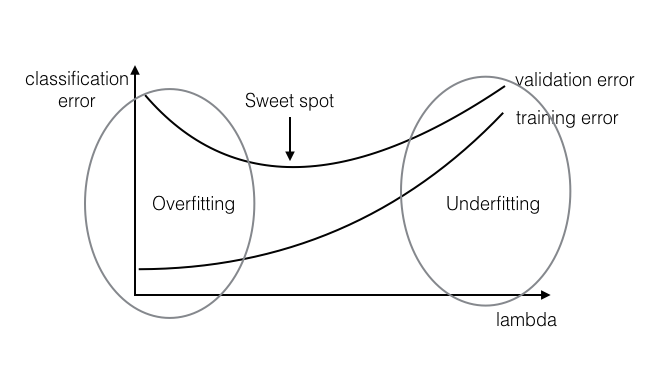
\includegraphics[scale=0.5]{pics/over-underfitting.png}
	\end{figure}
\end{frame}


\section{Identify the Sweet Spot}

%\subsection{Identify the Sweet Spot}
\begin{frame}
	\frametitle{Cross-Validation}
	\begin{block}{Cross-Validation}
		Divide data into training and validation portions. Train your algorithm on the "training" split and evaluate it on the "validation" split, for various value of $\lambda$ (Typical values: $10^{-5}$ $10^{-4}$ $10^{-3}$ $10^{-2}$ $10^{-1}$ $10^0$ $10^1$ $10^2$ ...).
	\end{block}
\end{frame}

\subsection{Cross-Validation}


\begin{frame}
	\frametitle{k-Fold Cross-Validation}
	Divide your training data into k partitions. Train on $k1$ of them and leave one out as validation set. Do this $k$ times (i.e. leave out every partition exactly once) and average the validation error across runs. This gives you a good estimate of the validation error (even with standard deviation). 
	\begin{figure}[h]
		\centering
		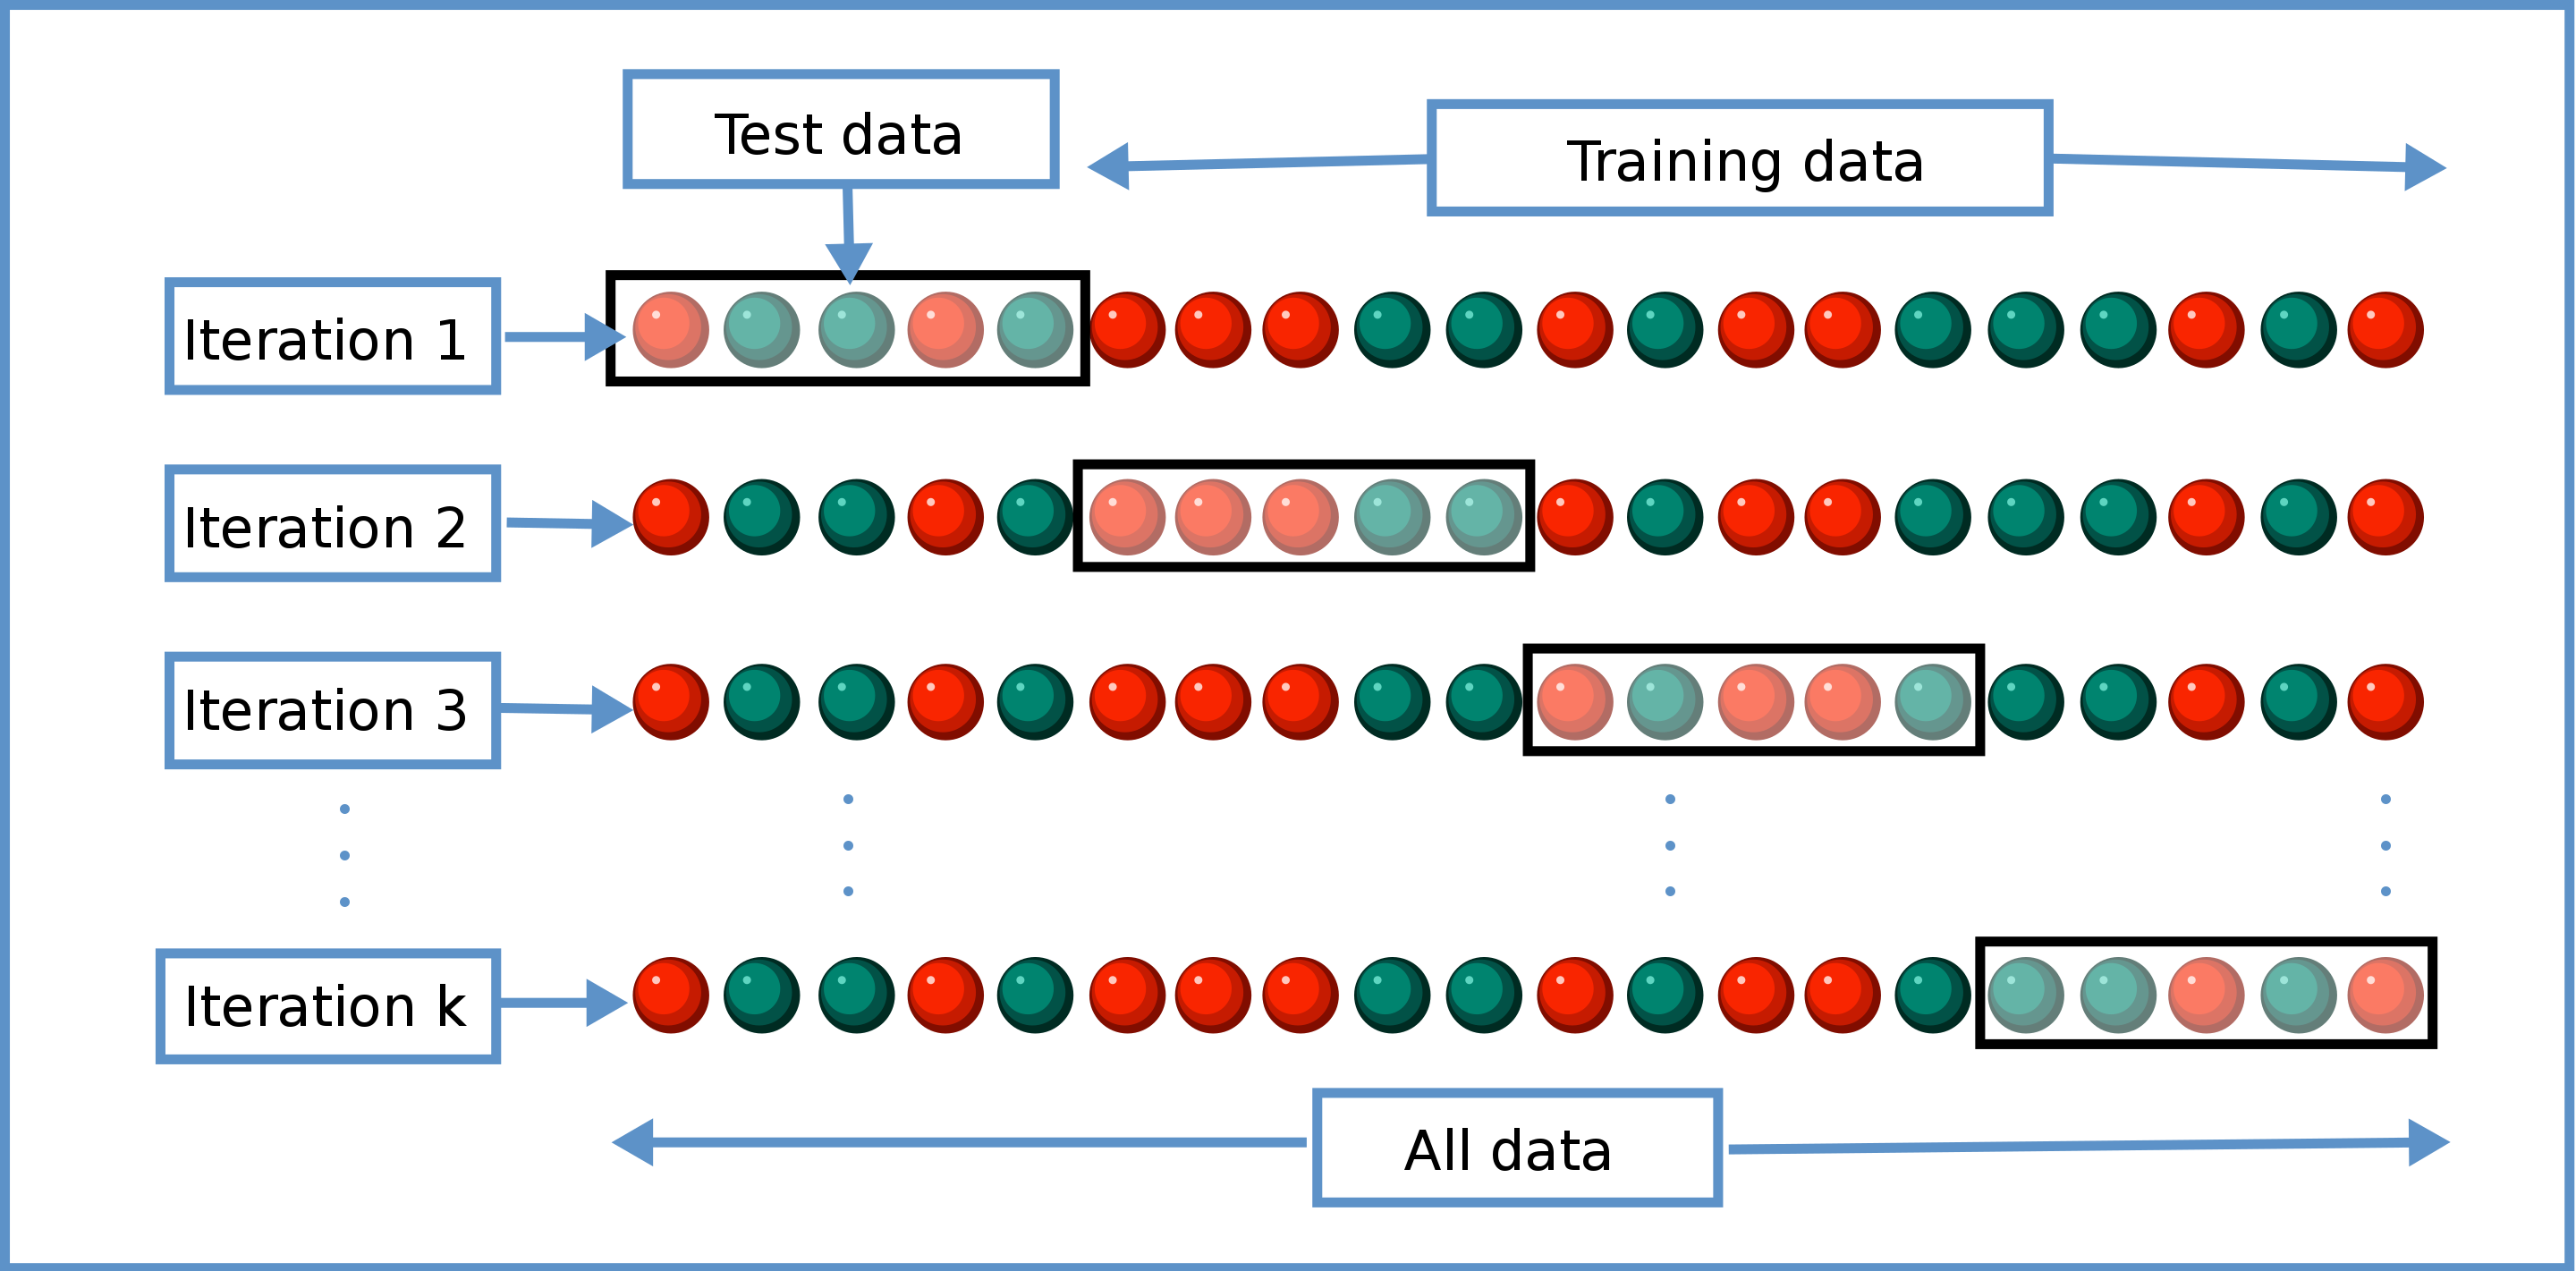
\includegraphics[scale=0.08]{pics/k-fold.png}
	\end{figure}
\end{frame}

\begin{frame}
	\frametitle{K-Fold Validation Error}
	\begin{block}{k-fold validation error}
		K-fold validation error is defined as:
		\begin{center}
			$\textbf{K-fold validation error}: \frac{1}{n} \sum_{k=1}^K \sum_{i\in D_k} \mathbf{1}(h(\mathbf{x}_i; D-D_k)\ne y_i)$
		\end{center}
		where $D-D_k$ is the dataset minus $k^{\text{th}}$ fold and $h(\mathbf{x}_i; D-D_k)$ is the classifier learned on $D-D_k$.
	\end{block}
\end{frame}

\begin{frame}
	\frametitle{Leave-One-Out Cross-Validation}
	In the extreme case, you can have k=n, i.e. you only leave a single data point out (this is often referred to as LOOCV- Leave One Out Cross Validation). LOOCV is important if your data set is small and cannot afford to leave out many data points for evaluation .
	
	\begin{block}{Leave-one-out error}
		Leave-one-out error is defined as:
		\begin{center}
			$\textbf{LOO error}: \frac{1}{n} \sum_i \mathbf{1}(h(\mathbf{x}_i; D_{-i})\ne y_i)$
		\end{center}
		where $D_{-i}$ is the dataset minus $i^{\text{th}}$ example and $h(\mathbf{x}_i; D_{-i})$ is the classifier learned on $D_{-i}$.
	\end{block}
\end{frame}

\subsection{Telescopic Search}
\begin{frame}
	\frametitle{Telescopic Search}
	\begin{block}{Telescopic Search}
		Do two searches: 
		\begin{itemize}
			\item
			1st, find the best order of magnitude for $\lambda$;
			\item
			2nd, do a more fine-grained search around the best $\lambda$ found so far.
		\end{itemize}
	\end{block}
	\begin{itemize}
		\item
		For example, first you try $\lambda = 0.01, 0.1, 1, 10, 100$. It turns out 10 is the best performing value.
		\item Then you try out $\lambda = 5, 10, 15, 20, 25,... , 95$ to test values "around" 10.
	\end{itemize}
	
\end{frame}

\section{Early Stopping}
\begin{frame}
	\frametitle{Early Stopping}
	Stop your optimization after $M$ ($\geq 0$) number of gradient steps, even if optimization has not converged yet.
	\begin{figure}[h]
		\centering
		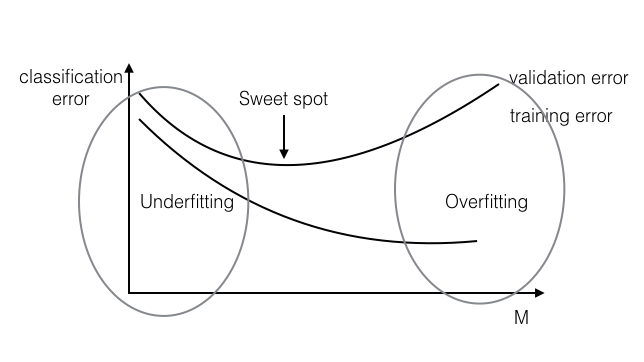
\includegraphics[scale=0.4]{pics/early-stopping.png}
	\end{figure}
\end{frame}

\begin{frame}
\Huge{\centerline{The End}}
\end{frame}
\end{CJK*}
\end{document}
%\end{document}
